\documentclass{standalone}
\usepackage{tikz}
\usepackage{float}
\usepackage{amsmath}
\usepackage{lmodern}
\usepackage{amssymb}
\usetikzlibrary{calc}
\usetikzlibrary{hobby}
\usetikzlibrary{decorations.markings}
\usetikzlibrary{patterns, patterns.meta}
\usetikzlibrary{shapes}

\begin{document}

\centering

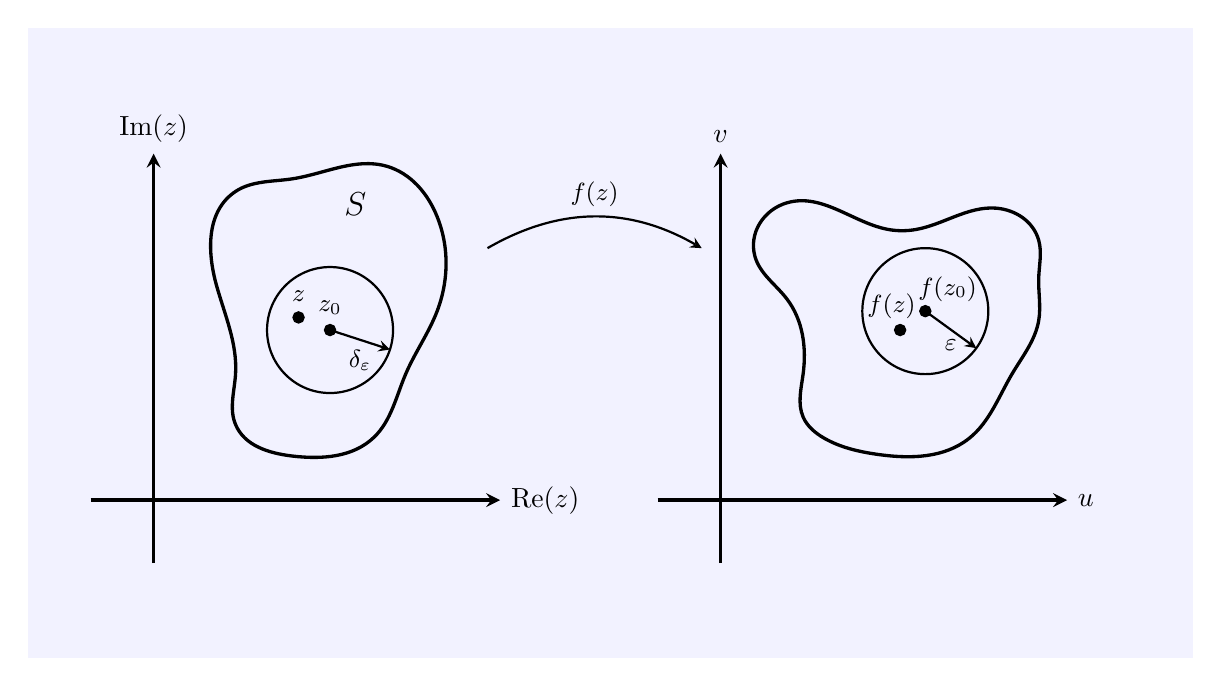
\begin{tikzpicture}[scale=0.80]
\pgfmathsetmacro{\CircleSize}{0.08}     % radius of coordinate circles/dots
% define styles used in this picture
\tikzset{
BigTextFont/.style={font=\large},
every node/.style={font=\small, text=black},
CircleNodeStyle/.style={draw=black, shape=circle, fill=black, minimum size=\CircleSize*1.8 cm, inner sep=0pt},
arrowstyle/.style={->, >=stealth}}

\colorlet{BlueBackground}{blue!5}
% Background for entire canvas
\fill[BlueBackground] (-3.5,-4.5) rectangle (15,5.5);

% Define function to draw axis of complex plane
\newcommand{\DrawAxes}[6]{%
  \pgfmathsetmacro{\OvershootAxis}{#1}%
  \pgfmathsetmacro{\AxisSize}{#2}%
  \pgfmathsetmacro{\XOriginAxis}{#3}%
  \pgfmathsetmacro{\YOriginAxis}{#4}%
  \draw[arrowstyle, very thick] (\XOriginAxis-\OvershootAxis,\YOriginAxis) -- (\XOriginAxis + \AxisSize,\YOriginAxis) node[pos=1, font=\normalsize, right] {#5};
  \draw[arrowstyle, very thick] (\XOriginAxis,\YOriginAxis-\OvershootAxis) -- (\XOriginAxis,\YOriginAxis + \AxisSize) node[pos=1, font=\normalsize, above] {#6};
}

%%% First subfigure: domain of the function with delta

\DrawAxes{1.0}{5.5}{-1.5}{-2.0}{$\mathrm{Re}(z)$}{$\mathrm{Im}(z)$}

% waypoint coordinates (in degrees, as seen from origin)
\begin{scope}[scale=1.0]
\coordinate (Odegrees) at (2.5,0);
\coordinate (20degrees) at (3,1);
\coordinate (40degrees) at (3,2.5);
\coordinate (55degrees) at (2.2,3.3);
\coordinate (80degrees) at (0.7,3.1);
\coordinate (95degrees) at (-0.2,2.9);
\coordinate (110degrees) at (-0.5,1.4);
\coordinate (180degrees) at (-0.2,0);
\coordinate (260degrees) at (-0.2,-0.8);
\coordinate (300degrees) at (0.7,-1.3);
\coordinate (330degrees) at (2.0,-1.0);
\end{scope}

\draw [very thick] (Odegrees) to[closed, curve through =
{(20degrees) (40degrees) (55degrees) (80degrees) (95degrees) (110degrees)  (180degrees) (260degrees) (300degrees) }] (330degrees);

% center of delta area
\coordinate (aLocation) at (1.3,0.7);   
\node [CircleNodeStyle, label=above:$z_0$] at (aLocation) {};

% random point z
\coordinate (zLocation) at ($(aLocation) + (-0.5,0.2)$);
\node [CircleNodeStyle, label=above:$z$] at (zLocation) {};

% create delta area
\draw[thick] 
[postaction={decorate}, decoration={
       markings,
       mark=at position 0.95 with {\node[name=EndVectorNode] {};}}]
(aLocation) circle [radius=1.0];

% draw radius of area
\draw[thick, arrowstyle]
[postaction={decorate}, decoration={
       markings,
       mark=at position 0.5 with {\node[name=EndVectorNode, below] {$\delta_{\varepsilon}$};}}] 
(aLocation) -- (EndVectorNode.center);

% domain symbol
\coordinate (DomainSymbolLoc) at (1.7,2.7);   
\node[ ellipse, inner sep=0, fill=BlueBackground, name=EndVectorNode, BigTextFont] at (DomainSymbolLoc) {$S$};

% transformation arrow
\draw[postaction={decorate}, decoration={markings,
mark=at position 0.5 with {\node[above] {$f(z)$};}}]
[arrowstyle, thick] (3.8, 2.0)  to[out=30,in=180-30] (7.2, 2.0);

%%% second subfigure: range of the function with delta

\begin{scope}[xshift=10.0cm]       % shift this whole subfigure to the right

% Call draw axes function
\DrawAxes{1.0}{5.5}{-2.5}{-2.0}{$u$}{$v$}


% waypoint coordinates (in degrees, as seen from origin)
\begin{scope}[scale=0.85]
\coordinate (Odegrees) at (2.5,0);
\coordinate (20degrees) at (3,1);
\coordinate (30degrees) at (3,1.8);
\coordinate (40degrees) at (3,2.5);
\coordinate (55degrees) at (2.2,3.1);
\coordinate (80degrees) at (0.7,2.7);
\coordinate (85degrees) at (0.2,2.7);
\coordinate (110degrees) at (-1.7,3.2);
\coordinate (125degrees) at (-2.3,2.2);
\coordinate (130degrees) at (-1.7,1.4);
\coordinate (180degrees) at (-1.4,0);
\coordinate (210degrees) at (-1.4,-0.8);
\coordinate (225degrees) at (-1.0,-1.2);
\coordinate (270degrees) at (0,-1.5);
\coordinate (330degrees) at (1.7,-1.2);
\end{scope}

% drawing area ("hobby" package)
\draw[very thick] (Odegrees) to[closed, curve through =
{ (20degrees) (30degrees) (40degrees) (55degrees) (80degrees) (85degrees) (110degrees) (125degrees) (130degrees)  (180degrees) (210degrees) (225degrees) (270degrees) }] (330degrees);

% f(zo) coordinate
\coordinate (fZOLocation) at (0.75,1.0);
\node [CircleNodeStyle] at (fZOLocation) {};
\node at ($(fZOLocation) + (45:5mm)$) {$f(z_0)$};

% point f(z)
\coordinate (fzLocation) at ($(fZOLocation) + (-0.4,-0.3)$);
\node [CircleNodeStyle] at (fzLocation) {};
\node at ($(fzLocation) + (110:4mm)$) {$f(z)$};

% create epsilon area
\draw[thick] 
[postaction={decorate}, decoration={
       markings,
       mark=at position 0.90 with {\node[name=EndVectorNode] {};}}]
(fZOLocation) circle [radius=1.0];

% draw radius of area
\draw[thick, arrowstyle]
[postaction={decorate}, decoration={
       markings,
       mark=at position 0.5 with {\node[name=EndVectorNode, below] {$\varepsilon$};}}] 
(fZOLocation) -- (EndVectorNode.center);


\end{scope}


\end{tikzpicture}

\end{document}